\chapter{Introdução}

\section{Contextualização}

A publicação de atos normativos é uma etapa fundamental do processo de gestão pública, pois formaliza e divulga para a sociedade as decisões do Governo Federal. A Receita Federal do Brasil\footnote{Disponível em \url{https://www.gov.br/receitafederal/pt-br}. Acesso em 06-jun-2021.} (RFB) disponibiliza atos normativos através do sistema Normas\footnote{Disponível em \url{http://normas.receita.fazenda.gov.br}. Acesso em 06-jun-2021.}, acessível publicamente através da Internet. Os atos são inicialmente publicados no Diário Oficial da União (DOU) através da Imprensa Nacional\footnote{Disponível em \url{https://www.in.gov.br/acesso-a-informacao/dados-abertos/base-de-dados}. Acesso em 06-jun-2021.} e incluídos manualmente no sistema Normas.

Um ato normativo é composto por segmentos, trechos que possuem um significado próprio definido pelo Decreto N\textsuperscript{o} 10.139 de 28 de novembro de 2019 \cite{Decreto10139} e formatação específica definida pelo Manual de Redação da Presidência de República \cite{ManualRedacao2018}. A figura \ref{fig:segmentos} apresenta um ato normativo destacando alguns segmentos de classes diferentes: a ementa destacada em vermelho, um inciso em azul, alguns artigos em verde e o fecho em marrom ao final do ato. 

\begin{figure}[h]
	\caption{Exemplo de Ato Normativos com Segmentos em Destaque}
	\center
	\label{fig:segmentos}
	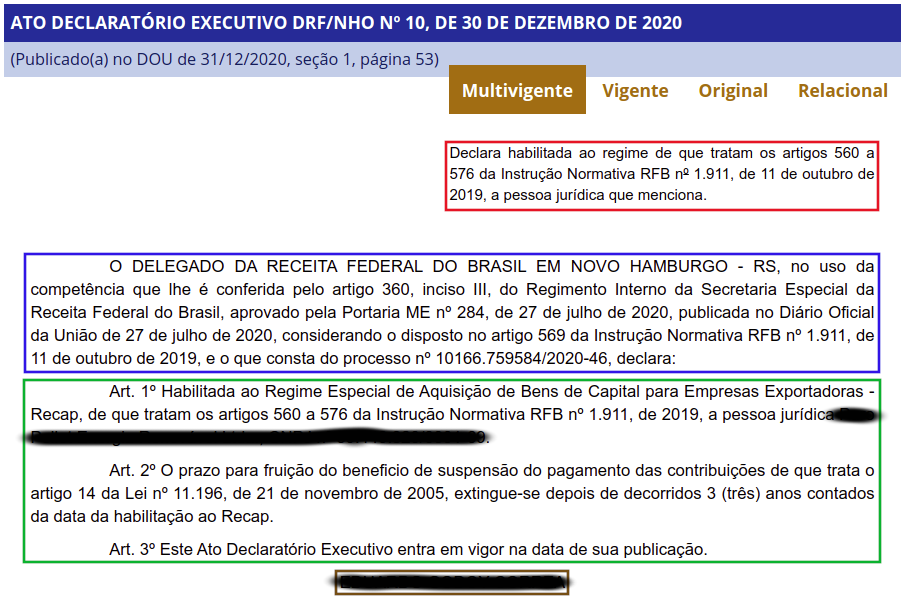
\includegraphics[scale=1.9]{introducao/segmentos.png}
\end{figure}

A classificação dos segmentos é uma etapa fundamental para o processo de inclusão de atos no sistema Normas, mas atualmente é realizada de forma totalmente manual, através de um procedimento que exige atenção e dedicação diária de uma equipe especializada da RFB. No período entre 2013 e 2020 foram incluídos aproximadamente 65 mil atos normativos compostos por mais de 600 mil segmentos, evidenciando um trabalho grande de classificação.

O Processamento de Linguagem Natural (PLN) é uma área da Ciência da Computação, fortemente relacionada com outras áreas como Inteligência Artificial e Aprendizagem de Máquina, que pesquisa métodos para analizar, modelar e compreender a linguagem humana \cite{PracticalNLP2020}. Uma das tarefas da PLN é a classificação de textos que consiste em atribuir uma classe previamente conhecida a um texto. Alguns exemplos de classificação de textos são a identificação de \textit{spam} em mensagens eletrônicas e a análise de sentimentos em comentários de redes sociais. Para o escopo desta pesquisa os textos são os segmentos dos atos normativos e as classes são os diferentes tipos de segmento a exemplo da ementa, do inciso, do artigo e do fecho. 

\section{O problema proposto}

Este trabalho propõe a criação de um modelo de aprendizado de máquina capaz de classificar automaticamente os segmentos de atos normativos provenientes do DOU, reduzindo o esforço e o tempo de inclusão dos atos no sistema Normas.     

